One purpose of mix networks is to provide untraceability to its
users. A mix-net takes as input a list of encrypted
messages. Verificatum is a reencryption mix-net. Such a mix-net
consists of a number of servers, mix servers, which sequentially
process the messages and reencrypts the list of messages and outputs
them in a randomized order. After passing through all servers, the
list of ciphertexts is decrypted and the result is a list of the
messages in random order.

In the context of electroinic voting a reencryption mix-nets may work
as follows.
\begin{enumerate}
\item The mix servers prepare the mix-net by generating public and
  secret keys.
\item Each voter encrypts his vote and appends it to a public list of
  encrypted votes.
\item In sequential order each mix server takes as input the list of
  encrypted votes, reencrypts and outputs them in a randomized order,
  replacing the previous list of encrypted votes.
\item After all mix servers have processed the list, each vote is
  jointly decrypted and posted on a bulletin board making the outcome
  of the election universally available without revealing how anyone
  voted.
\end{enumerate}

\begin{center}
  \makebox[\textwidth]{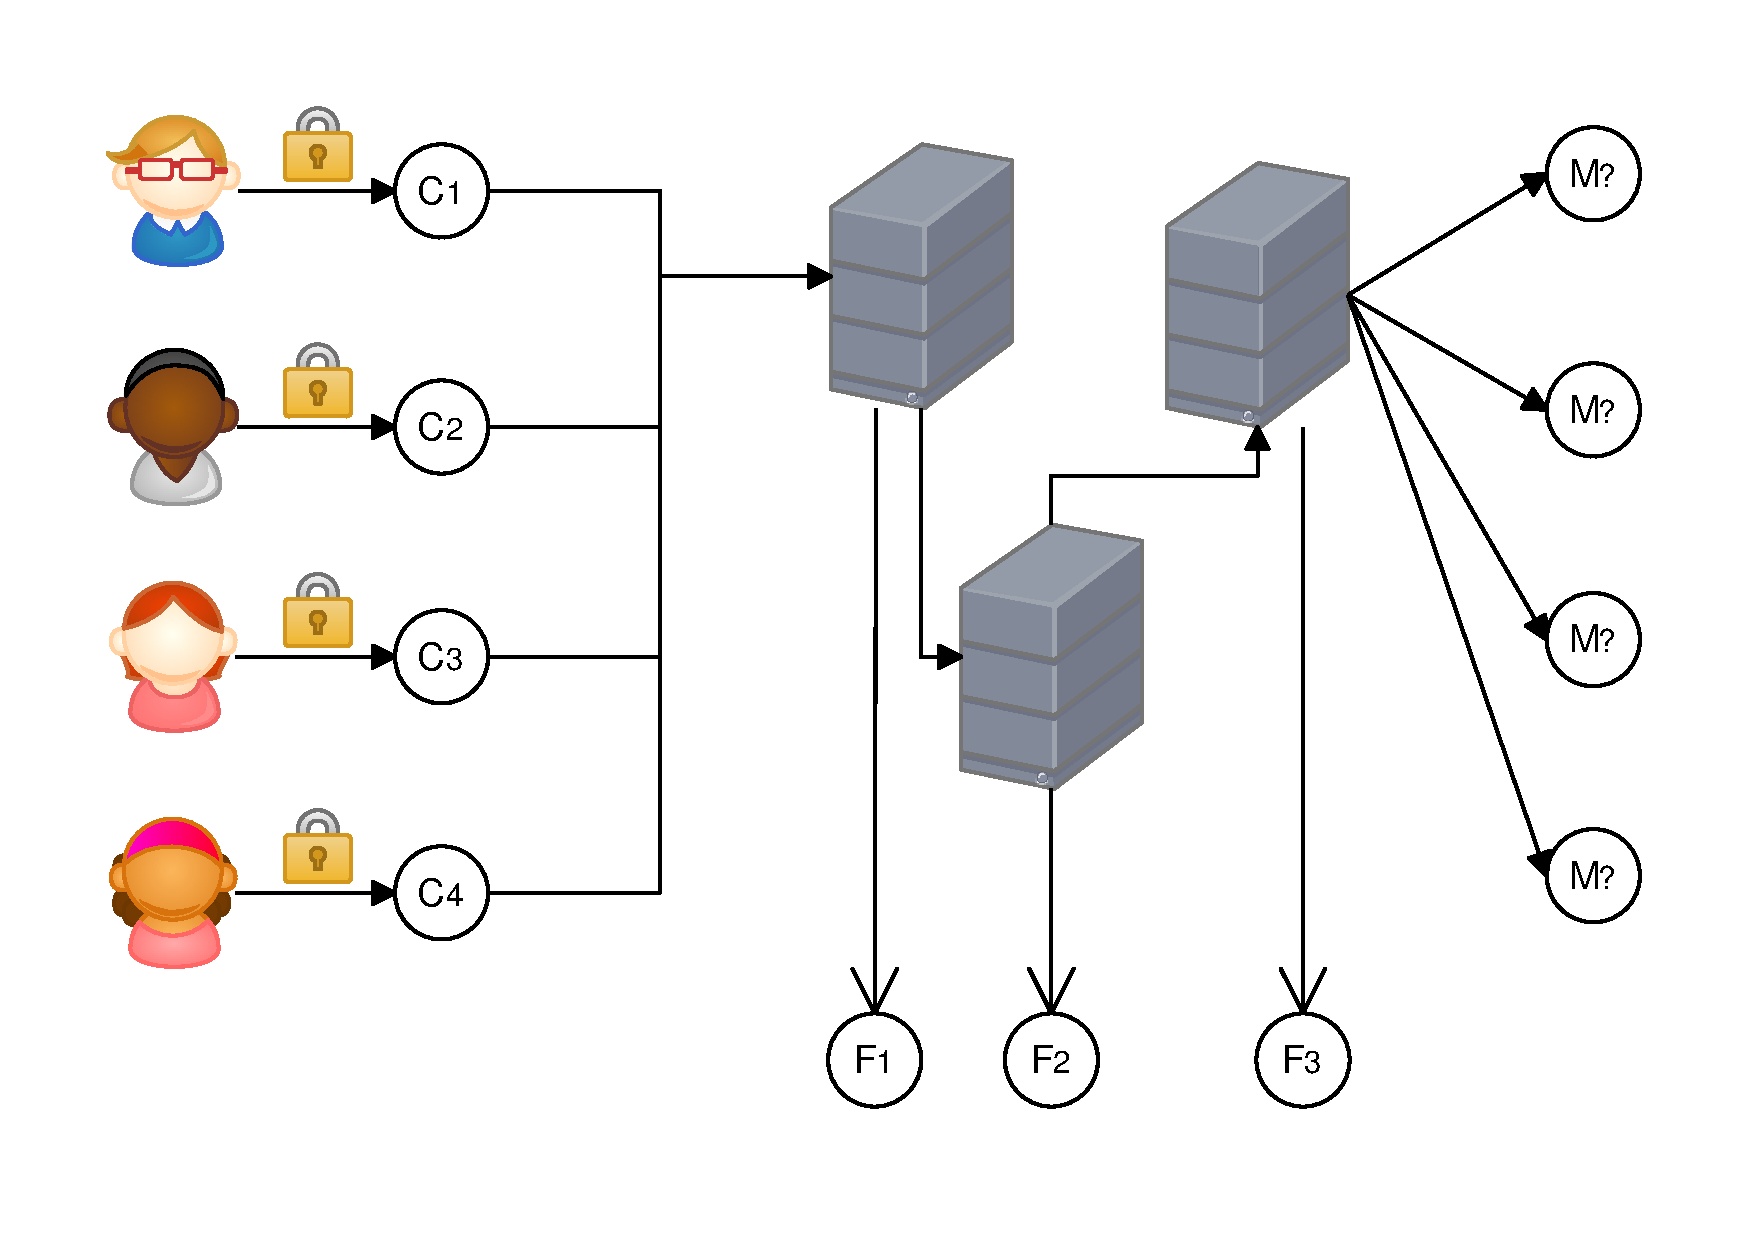
\includegraphics[width=\textwidth]{../presentation/images/mix2.pdf}}
\end{center}

